


\section{Data}
\label{sec-1}



Some time ago I found \url{http://www.nytimes.com/interactive/2009/03/10/us/20090310-immigration-explorer.html} (via
\url{http://www.smallmeans.com/new-york-times-infographics/}) and I wondered how a multivariate choropleth map could be
produced with R. Here is the code I have arranged to show the \url{http://en.wikipedia.org/wiki/Spanish_general_election,_2011} in a similar fashion.

Some packages are needed:


\lstset{language=R}
\begin{lstlisting}
library(maps)
library(maptools)
##gpclibPermit() ##needed for unionSpatialPolygons to work
##not needed if rgeos is installed
library(sp)
library(lattice)
library(latticeExtra)
library(colorspace)
\end{lstlisting}

Let's start with the data, which is available \url{http://dl.dropbox.com/u/40293713/spainVotes/votos2011.rda} (thanks to \url{http://uce.uniovi.es/~emilio/}, who ``massaged'' the original dataset, available from \url{http://www.infoelectoral.mir.es/docxl/04_201105_1.zip}).

Each region of the map will represent the percentage of votes obtained
by the predominant political option.  Besides, only four groups will
be considered: the two main parties (``PP'' and ``PSOE''), the abstention
results (``ABS''), and the rest of parties (``OTH'').


\lstset{language=R}
\begin{lstlisting}
load(url('http://dl.dropbox.com/u/40293713/spainVotes/votos2011.rda'))
votesData <- votos2011[, 12:1023] ##I don't need all the columns

votesData$ABS <- with(votos2011, Total.censo.electoral - Votos.validos) ##abstention

Max <- apply(votesData, 1, max)
whichMax <- apply(votesData,  1, function(x)names(votesData)[which.max(x)])

## OTH for everything but PP, PSOE and ABS
whichMax[!(whichMax %in% c('PP',  'PSOE', 'ABS'))] <- 'OTH'

## Finally, I calculate the percentage of votes with the electoral census
pcMax <- Max/votos2011$Total.censo.electoral * 100
\end{lstlisting}
\section{Administrative boundaries}
\label{sec-2}

The Spanish administrative boundaries are available as shapefiles at the \url{http://www.ine.es/ss/Satellite?c%3DPage&p%3D1254735116596&pagename%3DProductosYServicios%252FPYSLayout&cid%3D1254735116596&L%3D1} (\~{}70Mb):

\lstset{language=R}
\begin{lstlisting}
old <- setwd(tempdir())
download.file('http://goo.gl/TIvr4', 'mapas_completo_municipal.rar')
system2('unrar', c('e', 'mapas_completo_municipal.rar'))
espMap <- readShapePoly(fn="esp_muni_0109")
Encoding(levels(espMap$NOMBRE)) <- "latin1"

provinces <- readShapePoly(fn="spain_provinces_ag_2")
setwd(old)
\end{lstlisting}

  


\lstset{language=R}
\begin{lstlisting}
##There are some repeated polygons which can be dissolved with:
##gpclibPermit() ##needed for unionSpatialPolygons to work
espPols <- unionSpatialPolygons(espMap, espMap$PROVMUN) ##disolve repeated polygons
\end{lstlisting}

Spanish maps are commonly displayed with the Canarian islands next to
the peninsula. First we have to extract the polygons of the islands
and the polygons of the peninsula. 

\lstset{language=R}
\begin{lstlisting}
canarias <-  sapply(espPols@polygons, function(x)substr(x@ID, 1, 2) %in% c("35",  "38"))
peninsulaPols <- espPols[!canarias]
islandPols <- espPols[canarias]
\end{lstlisting}

Then we shift the coordinates of the islands with \texttt{elide}

\lstset{language=R}
\begin{lstlisting}
dy <- bbox(peninsulaPols)[2,1] - bbox(islandPols)[2,1]
dx <- bbox(peninsulaPols)[1,2] - bbox(islandPols)[1,2]

islandPols2 <- elide(islandPols, shift=c(dx, dy))
bbIslands <- bbox(islandPols2)
\end{lstlisting}

and finally construct a new \texttt{SpatialPolygons} object binding the
shifted islands with the peninsula.


\lstset{language=R}
\begin{lstlisting}
espPols <- rbind(peninsulaPols, islandPols2)
\end{lstlisting}

The last step before drawing the map is to link the data
with the polygons:

\lstset{language=R}
\begin{lstlisting}
IDs <- sapply(espPols@polygons, function(x)x@ID)
idx <- match(IDs, votos2011$PROVMUN)

##Places without information
idxNA <- which(is.na(idx))

##Information to be added to the SpatialPolygons object
dat2add <- data.frame(prov = votos2011$PROV,
                      poblacion = votos2011$Nombre.de.Municipio,
                      Max = Max,  pcMax = pcMax,  who = whichMax)[idx, ]

row.names(dat2add) <- IDs
espMapVotes <- SpatialPolygonsDataFrame(espPols, dat2add)

## Drop those places without information
espMapVotes <- espMapVotes[-idxNA, ]
\end{lstlisting}
\section{Map}
\label{sec-3}

So let's draw the map. I will produce a list of plots, one for
each group.  The \url{http://latticeextra.r-forge.r-project.org/#layer} of the \url{http://latticeextra.r-forge.r-project.org/#} package
with \texttt{Reduce} superposes the elements of this list and produce a
\texttt{trellis} object. I will use a set of sequential palettes from the
\url{http://cran.r-project.org/web/packages/colorspace/} package with a different \url{http://en.wikipedia.org/wiki/Hue} for each group.


\lstset{language=R}
\begin{lstlisting}
classes <- levels(factor(whichMax))
nClasses <- length(classes)

pList <- lapply(1:nClasses, function(i){
  mapClass <- espMapVotes[espMapVotes$who==classes[i],]
  step <- 360/nClasses ## distance between hues
  pal <- rev(sequential_hcl(16, h = (30 + step*(i-1))%%360)) ## hues equally spaced
  pClass <- spplot(mapClass['pcMax'], col.regions=pal, lwd=0.1,
                   at = c(0, 20, 40, 60, 80, 100))
  })

p <- Reduce('+', pList)
\end{lstlisting}
\subsection{Legend}
\label{sec-3-1}

However, the legend of this \texttt{trellis} object is not valid.  

First, a title for the legend of each element \texttt{pList} will be
useful. Unfortunately, the \texttt{levelplot} function (the engine under the
\texttt{spplot} method) does not allow for a title with its \texttt{colorkey}
argument. The \texttt{frameGrob} and \texttt{packGrob} of the \url{http://cran.r-project.org/web/packages/grid} package will do the work.


\lstset{language=R}
\begin{lstlisting}
addTitle <- function(legend, title){
  titleGrob <- textGrob(title, gp=gpar(fontsize=8), hjust=1, vjust=1)
  legendGrob <- eval(as.call(c(as.symbol(legend$fun), legend$args)))
  ly <- grid.layout(ncol=1, nrow=2, widths=unit(0.9, 'grobwidth', data=legendGrob))
  fg <- frameGrob(ly, name=paste('legendTitle', title, sep='_'))
  pg <- packGrob(fg, titleGrob, row=2)
  pg <- packGrob(pg, legendGrob, row=1)
  }

for (i in seq_along(classes)){
  lg <- pList[[i]]$legend$right
  lg$args$key$labels$cex=ifelse(i==nClasses, 0.8, 0) ##only the last legend needs labels
  pList[[i]]$legend$right <- list(fun='addTitle',
                                  args=list(legend=lg, title=classes[i]))
}
\end{lstlisting}

Now, every component of \texttt{pList} includes a legend with a title
below. The last step is to modify the legend of the \texttt{p} trellis object
in order to merge the legends from every component of \texttt{pList}.


\lstset{language=R}
\begin{lstlisting}
## list of legends
legendList <- lapply(pList, function(x){
  lg <- x$legend$right
  clKey <- eval(as.call(c(as.symbol(lg$fun), lg$args)))
  clKey
})

##function to pack the list of legends in a unique legend
##adapted from latticeExtra::: mergedTrellisLegendGrob
packLegend <- function(legendList){
  N <- length(legendList)
  ly <- grid.layout(nrow = 1,  ncol = N)
  g <- frameGrob(layout = ly, name = "mergedLegend")
  for (i in 1:N) g <- packGrob(g, legendList[[i]], col = i)
  g
}

## The legend of p will include all the legends
p$legend$right <- list(fun = 'packLegend',  args = list(legendList = legendList))
\end{lstlisting}
\subsection{Result}
\label{sec-3-2}


Here is the result with the provinces boundaries superposed (only for
the peninsula due to a problem with the definition of boundaries the Canarian
islands in the file) and a rectangle to separate the Canarian islands from the
rest of the map.


\lstset{language=R}
\begin{lstlisting}
canarias <- provinces$PROV %in% c(35, 38)
peninsulaLines <- provinces[!canarias,]

p +
  layer(sp.polygons(peninsulaLines,  lwd = 0.3)) +
  layer(grid.rect(x=bbIslands[1,1], y=bbIslands[2,1],
                  width=diff(bbIslands[1,]),
                  height=diff(bbIslands[2,]),
                  default.units='native', just=c('left', 'bottom'),
                  gp=gpar(lwd=0.5, fill='transparent')))
\end{lstlisting}

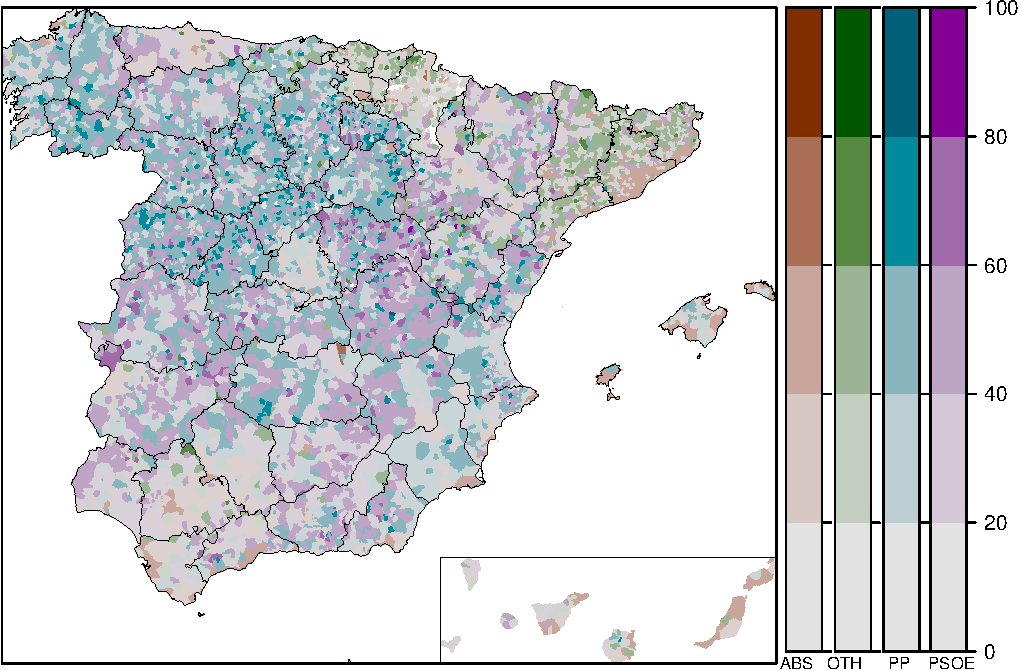
\includegraphics[width=.9\linewidth]{figs/mapLegends.pdf}
